\documentclass[12pt]{article}
\usepackage{fullpage}
\usepackage{graphicx}
\usepackage{booktabs}
\usepackage{tikz}
\usetikzlibrary{positioning, arrows.meta}
\setlength{\parskip}{5pt}
\setlength{\parindent}{0pt}

\begin{document}

\begin{center}
    {\Large \textbf{Predicting Formula 1 Race Results from Mid Race Features}}\\[4pt]
    Aditya Manoj Krishna (amkrishna@wpi.edu) \\
    Mehul Chandna (mmchandna@wpi.edu)
\end{center}

\section{Introduction}

This project predicts full Formula 1 race finishing orders using mid race information scraped and engineered from public HTML tables. The inputs include grid placement, pit stop timing, normalized fastest lap information, and one hot encoded team identity. The target is the complete ranking of all twenty drivers plus a DNF class. Predicting an entire race order is difficult because positions must form a strict permutation and because motorsport outcomes depend on many factors not contained in the scraped data. These include crashes, reliability issues, wind effects, strategy offsets, tire degradation, and safety cars. Despite these limitations the model consistently predicts realistic orderings within small position envelopes and produces strong ranking correlations, which shows that mid race features contain meaningful predictive structure.

\section{Data Collection}

Formula1.com does not provide lap by lap timing or sector deltas in its HTML pages. We therefore scraped four separate pages per race: the race result, the starting grid, the pit stop summary, and the fastest laps table. The site’s markup is not standardized across seasons, so we first extracted race links with a regular expression and then used a header matching strategy to locate tables even when column names differed slightly. Several tables had irregularities such as missing columns or textual status codes for retirements, so we repeatedly inspected raw HTML and updated our parsing logic until the scraper handled all seasons reliably.

Since the site provides only one lap time per driver we engineered derived pace features to compensate for the absence of full timing data. These included fastest lap rank, fastest lap lap fraction, and the time delta relative to the best lap of the event. Pit stop data required custom parsing because times sometimes appeared as mixed string formats. Retirements were converted into a single DNF label and races with fewer than twenty classified drivers were removed so that all tensors had consistent shape.

A significant amount of manual investigation was required to identify table structures, understand the meaning of ambiguous fields, resolve missing values, and transform irregular strings into numerical features. Constructing a reliable multi year dataset from this format was one of the more challenging parts of the project.

\section{Methods}

\subsection*{Feature engineering}

The final feature vector for each driver included normalized grid position, pit stop count, total pit time, first and last stop fractions, binary pitting indicators, normalized fastest lap rank, fastest lap fraction, fastest lap delta, and one hot team encoding. These features were chosen to act as coarse approximations for race pace and strategy since full telemetry was unavailable. For each race we produced a tensor of shape \([20, F]\) representing all driver feature vectors and paired it with the true finishing order.

\subsection*{Model}

We began with a simple binary winner classifier to confirm that the features carried usable signal, then moved to a multilayer perceptron that predicted independent finishing positions. This independent model frequently assigned the same position to multiple drivers, which revealed the need for a structured output method.

The final model applies an MLP to each driver and outputs scores for positions one to twenty and DNF. To convert these scores into a coherent race ordering we used the Hungarian algorithm to compute a one to one assignment between drivers and finishing positions. DNFs were then relocated to the bottom and remaining positions were re indexed. This structured assignment step was essential for obtaining realistic race order predictions.

Training used focal loss with class weighting so that DNF cases, which are comparatively rare, were not ignored. We tuned hyperparameters through five fold cross validation and recorded parameter trajectories to visualize the loss landscape \(f(\theta)\). We also visualized the prediction surface \(g(x)\) by performing PCA on driver features and mapping changes in feature space to changes in expected finishing position.

\subsection*{Podium focused metric}

To better evaluate high value positions we added a podium penalty metric that measures accuracy within plus or minus two positions for true podium drivers and treats any model predicted DNF for a podium finisher as a severe error. This reflects how race outcomes are judged in practice and gives meaningful insight into model performance at the front of the grid.

\section{Results}

Table \ref{tab:results} summarizes the final results on the held out test set of forty one races. Exact match accuracy is low because full permutation prediction is inherently difficult, so we rely on structured metrics that reflect how close the predicted order is to the real finishing order.

The model places 36.1 percent of drivers within one position of their true finish, 52.4 percent within two positions, and 67.9 percent within three positions. These envelopes show that even without telemetry the model reconstructs much of the race structure. Kendall's \(\tau\) and Spearman's \(\rho\) were both high, which indicates strong agreement between the predicted and true rankings across entire grids. NDCG was also high which shows that the front of the field is modeled reliably even when predictions for the backmarkers vary. The podium penalty metric showed that the model rarely mislabels genuine frontrunners as DNFs and usually predicts podium finishes within two positions.

Pairwise ordering accuracy and displacement at small values of \(k\) provided additional structure aware evaluation. These metrics show that the model usually orders driver pairs correctly and rarely misplaces top contenders by large margins.

\begin{table}[h]
    \centering
    \caption{Final model performance}
    \label{tab:results}
    \begin{tabular}{lc}
        \toprule
        Metric & Value \\
        \midrule
        Accuracy plus or minus one & 36.10 percent \\
        Accuracy plus or minus two & 52.44 percent \\
        Accuracy plus or minus three & 67.93 percent \\
        Kendall's $\tau$ & 0.5741 \\
        Spearman's $\rho$ & 0.7344 \\
        NDCG all & 0.8269 \\
        Podium within two positions & 64.3 percent \\
        Podium DNF error rate & 3.1 percent \\
        Pairwise ordering accuracy & 81.7 percent \\
        \bottomrule
    \end{tabular}
\end{table}

\subsection*{Loss landscape visualization}  
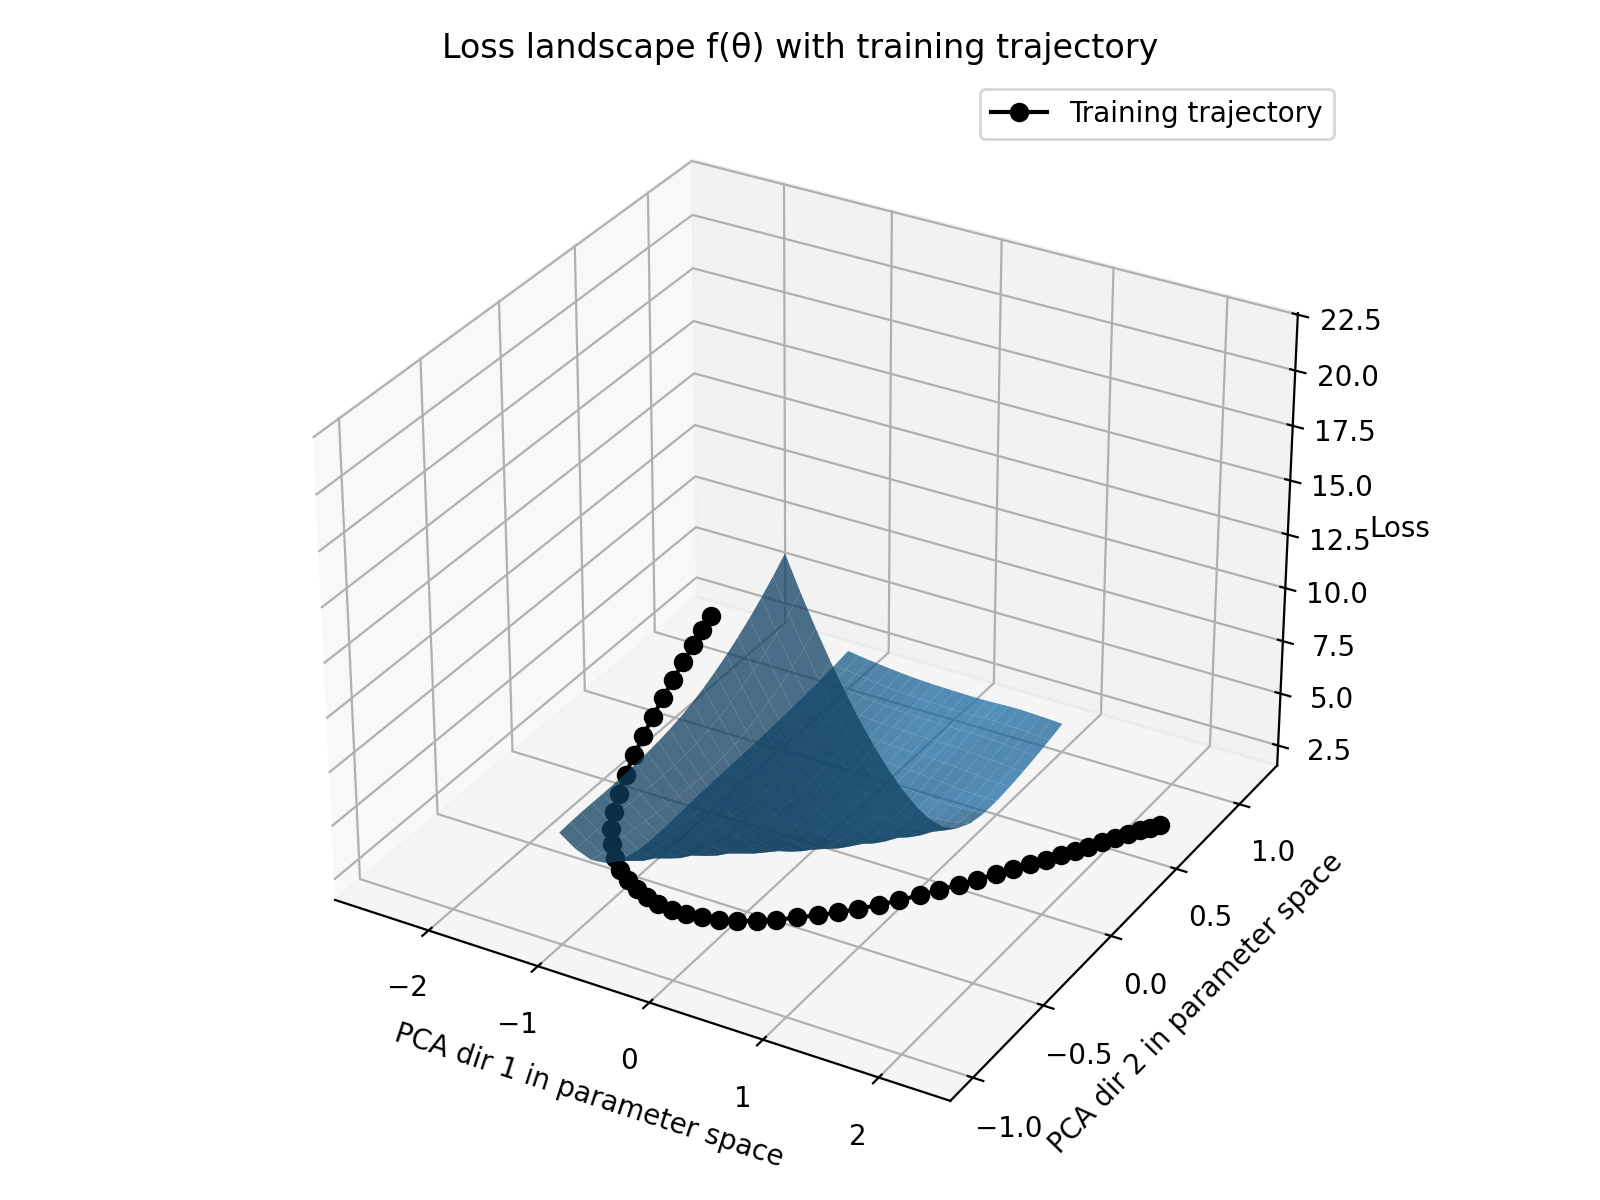
\includegraphics[width=\linewidth]{loss_landscape_f_theta.png}

\subsection*{Prediction surface visualization}  
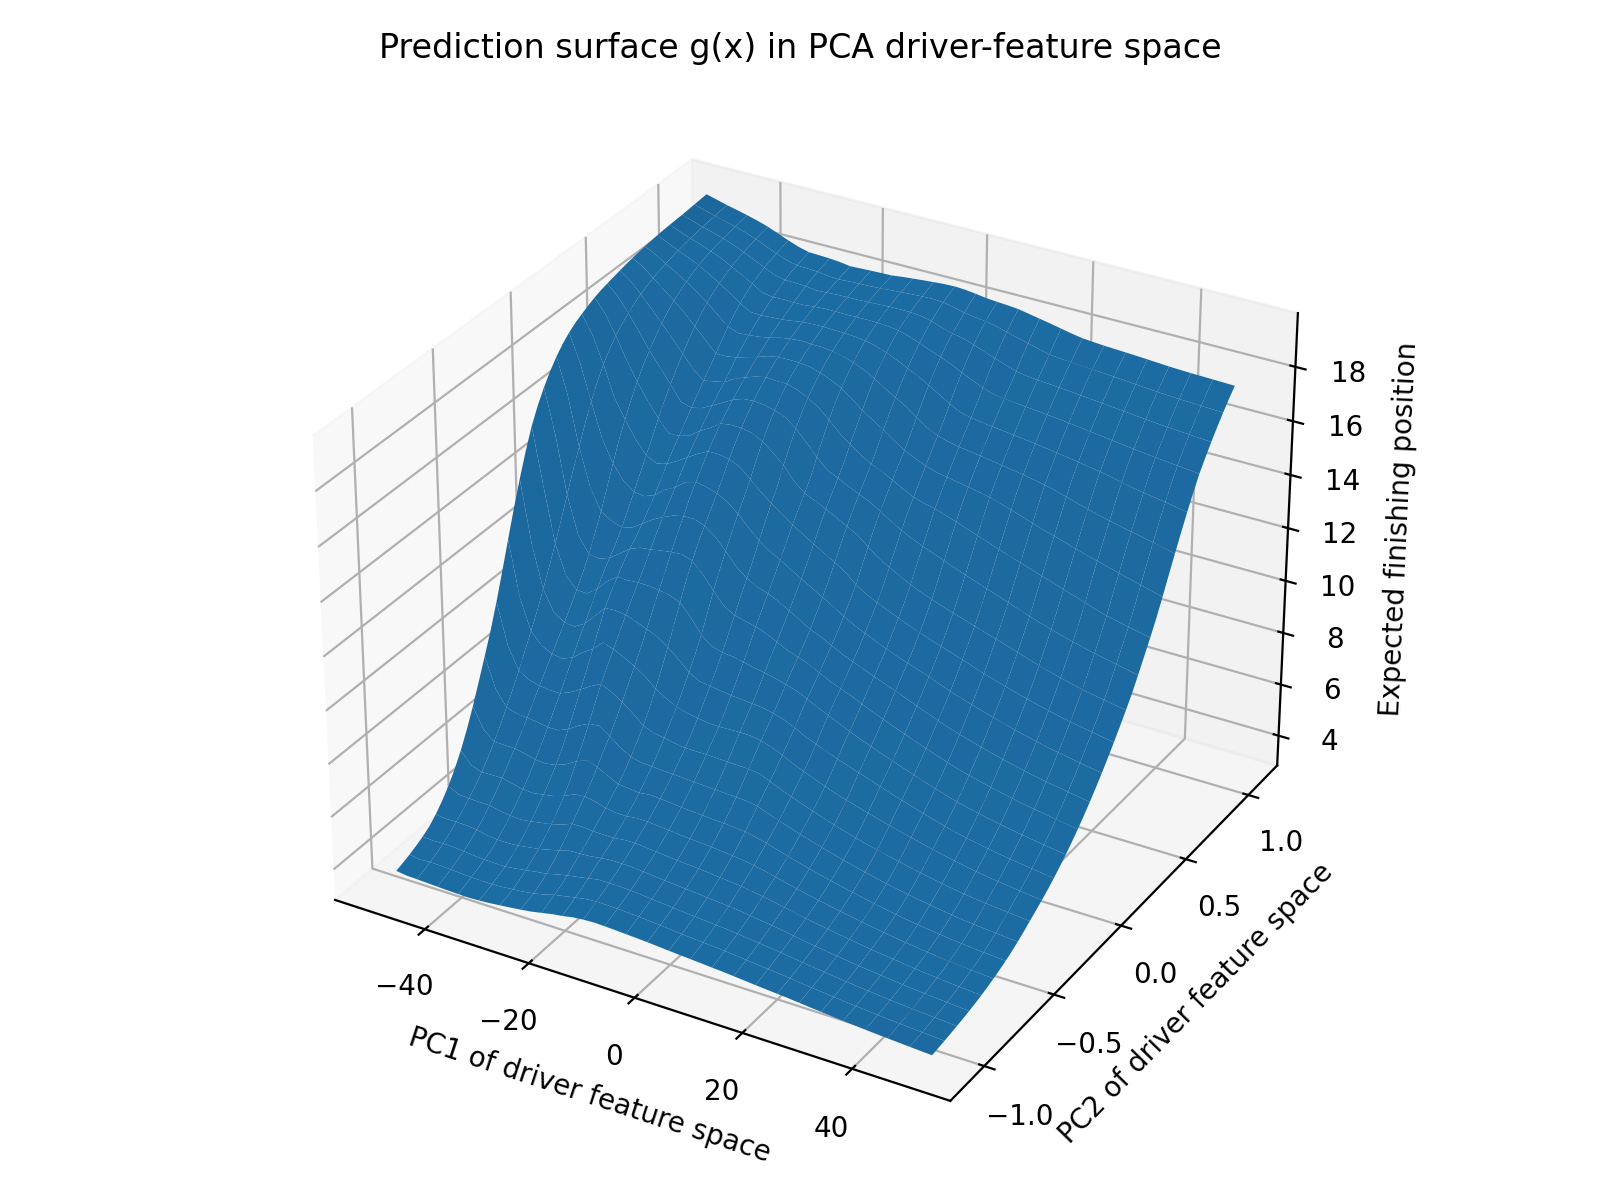
\includegraphics[width=\linewidth]{prediction_surface_g_x.png}

\section{Challenges and solutions}

The project required several nontrivial solutions. The lack of lap by lap timing forced us to design pace features from only a single lap, which required careful normalization across races and seasons. HTML inconsistencies demanded repeated manual inspection and revision of scraping logic. Handling DNFs was particularly complex because the site encodes retirements using multiple textual formats. Treating these inconsistently produced unstable training signals until we unified them into a single label and filtered incomplete races.

Independent position prediction models often produced impossible outputs with duplicate positions, which led us to adopt a structured assignment method. Incorporating the Hungarian algorithm and postprocessing logic significantly improved coherence. Finally, evaluating permutation predictions required more than a single accuracy number, so we developed a metric suite that included ranking correlations, envelope accuracy, pairwise ordering statistics, and a podium sensitive measure. These metrics provided a realistic view of model behavior and were essential for guiding improvements.

\section{Conclusions}

Even with limited mid race data the final model captures much of the predictable structure in Formula 1 racing. Grid placement, pit timing, and fastest lap derived pace indicators provided enough information to reconstruct a large portion of the final standings. The strongest engineering steps were building useful features from sparse data, resolving DNF inconsistencies, and enforcing permutation structure through the Hungarian algorithm. The metric suite showed that the model performs well where it matters most: it preserves ranking structure, predicts frontrunners reliably, and makes few severe errors for podium contenders. The project demonstrates that meaningful race order prediction is possible even when only high level mid race summaries are available.

\section*{Appendix: ChatGPT Prompt and Response}

https://chatgpt.com/share/6937450c-3968-800f-82c4-fe1aa16f16b2

\section{Neural Network Diagram}

\begin{figure}[h]
\centering
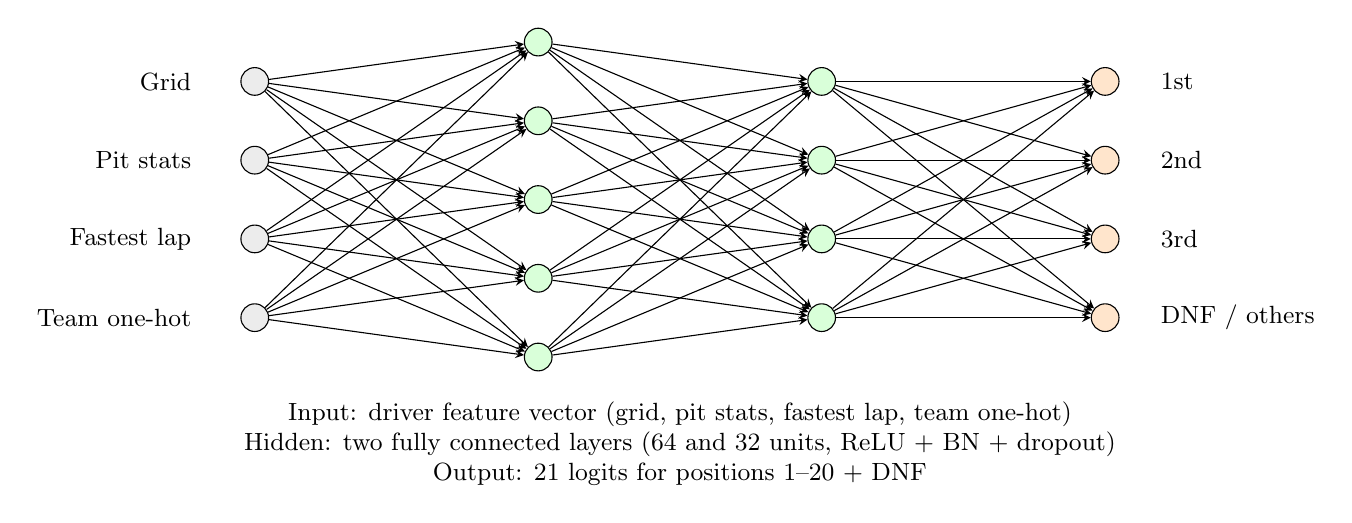
\begin{tikzpicture}[
    x=1.8cm,
    y=1.0cm,
    >=stealth,
    neuron/.style={circle, draw, minimum size=10pt, inner sep=0pt},
    every node/.style={font=\small}
]

%---------------- Input layer ----------------
\foreach \name/\y in {I1/1.5, I2/0.5, I3/-0.5, I4/-1.5} {
    \node[neuron, fill=gray!15] (\name) at (0,\y) {};
}
\node[left=0.5cm of I1, align=right] {Grid};
\node[left=0.5cm of I2, align=right] {Pit stats};
\node[left=0.5cm of I3, align=right] {Fastest lap};
\node[left=0.5cm of I4, align=right] {Team one-hot};

%---------------- Hidden layer 1 (64 units) ----------------
\foreach \name/\y in {H11/2.0, H12/1.0, H13/0.0, H14/-1.0, H15/-2.0} {
    \node[neuron, fill=green!15] (\name) at (2,\y) {};
}


%---------------- Hidden layer 2 (32 units) ----------------
\foreach \name/\y in {H21/1.5, H22/0.5, H23/-0.5, H24/-1.5} {
    \node[neuron, fill=green!15] (\name) at (4,\y) {};
}


%---------------- Output layer (21 logits) ----------------
\foreach \name/\y/\lab in {O1/1.5/{1st}, O2/0.5/{2nd}, O3/-0.5/{3rd}, O4/-1.5/{DNF / others}} {
    \node[neuron, fill=orange!20] (\name) at (6,\y) {};
    \node[right=0.4cm of \name] {\lab};
}


%---------------- Connections ----------------
\foreach \i in {1,...,4} {
    \foreach \j in {1,...,5} {
        \draw[->] (I\i) -- (H1\j);
    }
}

\foreach \i in {1,...,5} {
    \foreach \j in {1,...,4} {
        \draw[->] (H1\i) -- (H2\j);
    }
}

\foreach \i in {1,...,4} {
    \foreach \j in {1,...,4} {
        \draw[->] (H2\i) -- (O\j);
    }
}
\node at (3,-3.1) [align=center] {
  Input: driver feature vector (grid, pit stats, fastest lap, team one-hot)\\
  Hidden: two fully connected layers (64 and 32 units, ReLU + BN + dropout)\\
  Output: 21 logits for positions 1--20 + DNF
};
\end{tikzpicture}

\caption{Neural network used for per-driver scoring. The model ingests a driver feature vector and produces 21 logits, which are converted to a valid race order through the Hungarian assignment.}
\end{figure}

\end{figure}

\end{document}
